%杨舒云的实验报告编辑界面,使用了Huanyu Shi,2019级的模板,杨舒云在此拜谢ORZ!

%!TEX program = xelatex
\documentclass[dvipsnames, svgnames,a4paper,11pt]{article}
% ----------------------------------------------------- 
%	加边框的命令
%	参考:https://tex.stackexchange.com/questions/531559/how-to-add-the-page-border-for-first-two-pages-in-latex
\usepackage{tikz}
\usetikzlibrary{calc}
\usepackage{eso-pic}
\AddToShipoutPictureBG{%
\begin{tikzpicture}[overlay,remember picture]
\draw[line width=0.6pt] % 边框粗细
    ($ (current page.north west) + (0.6cm,-0.6cm) $)
    rectangle
    ($ (current page.south east) + (-0.6cm,0.6cm) $); % 边框位置
\end{tikzpicture}}


\usepackage{xcolor}
\definecolor{c1}{HTML}{086173} % 目录颜色 原版为2752C9 紫灰色535AAA 蓝紫色0B0DB7 深蓝色070F94 湖绿色219394 松石灰绿086173
\definecolor{c2}{HTML}{E20129} % 引用颜色 原版\definecolor{c2}{RGB}{190,20,83} 橙色F24729

\usepackage{ctex}
\usepackage[top=28mm,bottom=28mm,left=15mm,right=15mm]{geometry}
\usepackage{hyperref} 
\hypersetup{
	colorlinks,
	linktoc = section, % 超链接位置,选项有section, page, all
	linkcolor = c1, % linkcolor 目录颜色
	citecolor = c1  % citecolor 引用颜色
}
\usepackage{amsmath,enumerate,multirow,float}
\usepackage{tabularx}
\usepackage{tabu}
\usepackage{subfig}
\usepackage{fancyhdr}
\usepackage{graphicx}
\usepackage{wrapfig}  
\usepackage{physics}
\usepackage{appendix}
\usepackage{amsfonts}

%
\usepackage{tcolorbox}
\tcbuselibrary{skins,breakable}
\newtcolorbox{tbox}[2][]{
    colframe=black!70!,
    breakable,
    enhanced,
	boxrule =0.5pt,
    title = {#2},
    fonttitle = \large\kaishu\bfseries,
	drop fuzzy shadow,
    #1
}
\newtcolorbox[auto counter,number within=section]{question}[1][]{
  top=2pt,bottom=2pt,arc=1mm,
  boxrule=0.5pt,
%   frame hidden,
  breakable,
  enhanced, %跨页后不会显示下边框
  coltitle=c1!80!gray,
  colframe=c1,
  colback=c1!3!white,
  drop fuzzy shadow,
  title={思考题~\thetcbcounter:\quad},
  fonttitle=\bfseries,
  attach title to upper,
  #1
}

% ---------------------------------------------------------------------
%	利用cleveref改变引用格式,\cref是引用命令
\usepackage{cleveref}
\crefformat{figure}{#2{\textcolor{c2}{Figure #1}}#3} % 图片的引用格式
\crefformat{equation}{#2{(\textcolor{c2}{#1})}#3} % 公式的引用格式
\crefformat{table}{#2{\textcolor{c2}{Table #1}}#3} % 表格的引用格式


% ---------------------------------------------------------------------
%	页眉页脚设置
\fancypagestyle{plain}{\pagestyle{fancy}}
\pagestyle{fancy}
\lhead{\kaishu 中山大学物理与天文学院电子技术实验\uppercase\expandafter{\romannumeral1}} % 左边页眉,学院 + 课程
\rhead{\kaishu 实验报告By杨舒云\&戴鹏辉} % 右边页眉,实验报告标题
\cfoot{\thepage} % 页脚,中间添加页码


% ---------------------------------------------------------------------
%	对目录、章节标题的设置
\renewcommand{\contentsname}{\centerline{\huge 目录}}
\usepackage{titlesec}
\usepackage{titletoc}
% \titleformat{章节}[形状]{格式}{标题序号}{序号与标题间距}{标题前命令}[标题后命令]
\titleformat{\section}{\centering\LARGE\songti}{}{1em}{}

% ---------------------------------------------------------------------
%   listing代码环境设置
\usepackage{listings}
\lstloadlanguages{python}
\lstdefinestyle{pythonstyle}{
backgroundcolor=\color{gray!5},
language=python,
frameround=tftt,
frame=shadowbox, 
keepspaces=true,
breaklines,
columns=spaceflexible,                   
basicstyle=\ttfamily\small, % 基本文本设置,字体为teletype,大小为scriptsize
keywordstyle=[1]\color{c1}\bfseries, 
keywordstyle=[2]\color{Red!70!black},   
stringstyle=\color{Purple},       
showstringspaces=false,
commentstyle=\ttfamily\scriptsize\color{green!40!black},%注释文本设置,字体为sf,大小为smaller
tabsize=2,
morekeywords={as},
morekeywords=[2]{np, plt, sp},
numbers=left, % 代码行数
numberstyle=\it\tiny\color{gray}, % 代码行数的数字字体设置
stepnumber=1,
rulesepcolor=\color{gray!30!white}
}




% ---------------------------------------------------------------------
%	其他设置
\def\degree{${}^{\circ}$} % 角度
\graphicspath{{./images/}} % 插入图片的相对路径
\allowdisplaybreaks[4]  %允许公式跨页 
\usepackage{lipsum}
\usepackage{adjustbox}
%\usepackage{mathrsfs} % 字体
\captionsetup[figure]{name=Figure} % 图片形式
\captionsetup[table]{name=Table} % 表格形式

\begin{document}
	
	
	
	% 实验报告封面	
	
	% 顶栏
	\begin{table}
		\renewcommand\arraystretch{1.7}
		\begin{tabularx}{\textwidth}{
				|X|X|X|X
				|X|X|X|X|}
			\hline
			\multicolumn{2}{|c|}{预习报告}&\multicolumn{2}{|c|}{实验记录}&\multicolumn{2}{|c|}{分析讨论}&\multicolumn{2}{|c|}{总成绩}\\
			\hline
			\LARGE25 & & \LARGE25 & & \LARGE30 & & \LARGE80 & \\
			\hline
		\end{tabularx}
	\end{table}
	% ---
	
	% 信息栏
	\begin{table}
		\renewcommand\arraystretch{1.7}
		\begin{tabularx}{\textwidth}{|X|X|X|X|}
			\hline
			年级、专业: & 2022级 物理学 &组号: & 2\\
			\hline
			姓名: & 戴鹏辉、杨舒云  & 学号: & 22344016、22344020\\
			\hline
			实验时间: & 2024/6/19 & 教师签名: & \\
			\hline
		\end{tabularx}
	\end{table}
	% ---
	
	% 大标题
	\begin{center}
		\LARGE ET1-11 \quad 模拟运算放大电路
	\end{center}
	% ---
	
	% 注意事项
	
	% 基本
	\textbf{【实验报告注意事项】}
	\begin{enumerate}
		\item 实验报告由三部分组成:
		\begin{enumerate}
			\item 预习报告:课前认真研读实验讲义,弄清实验原理;实验所需的仪器设备、用具及其使用、完成课前预习思考题;了解实验需要测量的物理量,并根据要求提前准备实验记录表格(可以参考实验报告模板,可以打印)。\textcolor{red}{\textbf{(20分)}}
			\item 实验记录:认真、客观记录实验条件、实验过程中的现象以及数据。实验记录请用珠笔或者钢笔书写并签名(\textcolor{red}{\textbf{用铅笔记录的被认为无效}})。\textcolor{red}{\textbf{保持原始记录,包括写错删除部分,如因误记需要修改记录,必须按规范修改。}}(不得输入电脑打印,但可扫描手记后打印扫描件);离开前请实验教师检查记录并签名。\textcolor{red}{\textbf{(30分)}}
			\item 数据处理及分析讨论:处理实验原始数据(学习仪器使用类型的实验除外),对数据的可靠性和合理性进行分析;按规范呈现数据和结果(图、表),包括数据、图表按顺序编号及其引用;分析物理现象(含回答实验思考题,写出问题思考过程,必要时按规范引用数据);最后得出结论。\textcolor{red}{\textbf{(30分)}}
		\end{enumerate}
		\textbf{实验报告就是将预习报告、实验记录、和数据处理与分析合起来,加上本页封面。\textcolor{red}{(80分)}}
		\item 每次完成实验后的一周内交\textbf{实验报告}(特殊情况不能超过两周)。
		\item \textbf{其它注意事项}:
		\begin{enumerate}
			\item 请认真查看并理解实验讲义第一章内容;
			\item 注意实验器材的合理使用;
			\item 使用结束使用各种仪器之后需要将其放回原位。
		\end{enumerate}
	\end{enumerate}
	
	% 安全
	%\textbf{【实验安全注意事项】}	
	
	
	% ---
	
	% 特别鸣谢
	\textbf{【特别鸣谢及模板说明】}	
	
	感谢2019级学长石寰宇为本实验报告提供\LaTeX 模板。\textcolor{red}{\textbf{由于原实验报告模板缺少实验编号,为方便在电脑上整理,故添加自命名编号ET1-11。}}
	% ---
	
	
	
	% 目录
	\clearpage
	\tableofcontents
	\clearpage
	% ---
	
	
	
	% 预习报告	
	
	% 小标题
	\setcounter{section}{0}
	\section{ET1-11 模拟运算放大电路 \quad\heiti 预习报告}
	% ---
	
	% 实验目的
	\subsection{实验目的}
	\begin{enumerate}
		\item 了解运算放大器的基本使用方法。
		\item 应用集成运放构成基本运算电路,并测定它们输出信号与输入信号间运算关系。
		\item 学会使用线性组件741运放。 		
	\end{enumerate}
	% ---
	
	\begin{figure}[htbp]
		\centering
		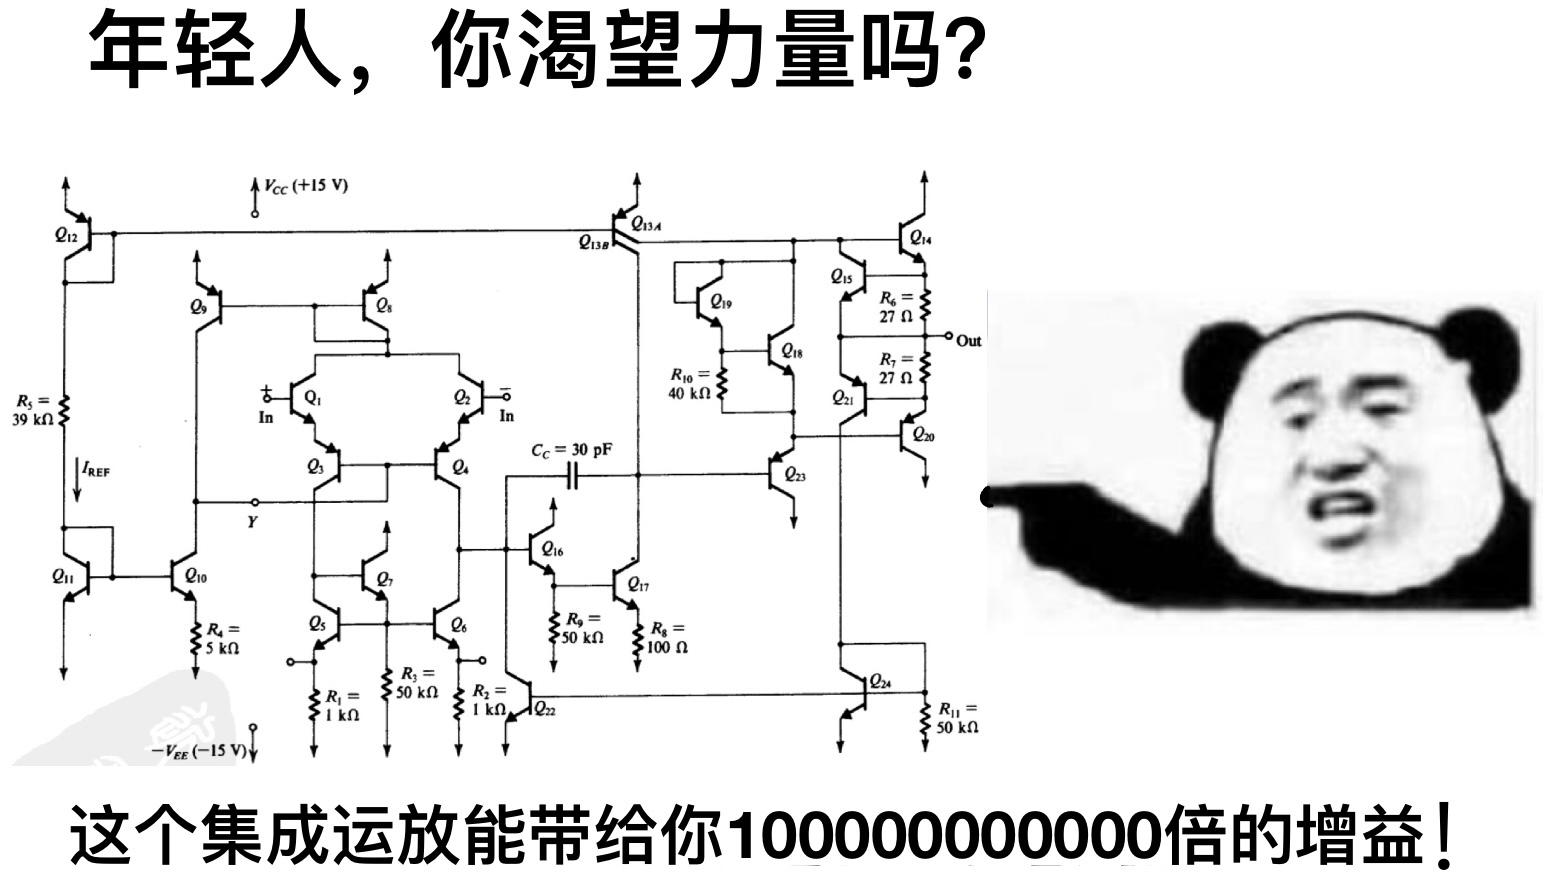
\includegraphics[width=0.7\textwidth]{ET1_11GraP1.png}
		\caption{741运放内部结构展示}
		\label{fig:figP1}
	\end{figure}
	
	% 仪器用具
	\subsection{仪器用具}
	\begin{table}[htbp]
		\centering
		\renewcommand\arraystretch{1.6}
		% \setlength{\tabcolsep}{10mm}
		\begin{tabular}{p{0.05\textwidth}|p{0.20\textwidth}|p{0.05\textwidth}|p{0.5\textwidth}}
			\hline
			编号& 仪器用具名称 & 数量 &  主要参数(型号,测量范围,测量精度等) \\
			\hline
			1&  电路原理箱或板& 1 &  \\
			\hline
			2&  函数信号发生器& 1 &  \\
			\hline
			3&  交流毫伏表& 1 &  \\
			\hline
			4&  数字万用表& 1 &  \\
			\hline
			5&  双踪示波器& 1 &  \\
			\hline
		\end{tabular}
	\end{table}
	% ---
	
	% 原理概述
	\subsection{原理概述}
	根据运放得基本原理,我们对实验所用的几种电路得闭环增益(及相关量)得理论值进行了计算,结果如图所示。
	
	\begin{figure}[htbp]
		\centering
		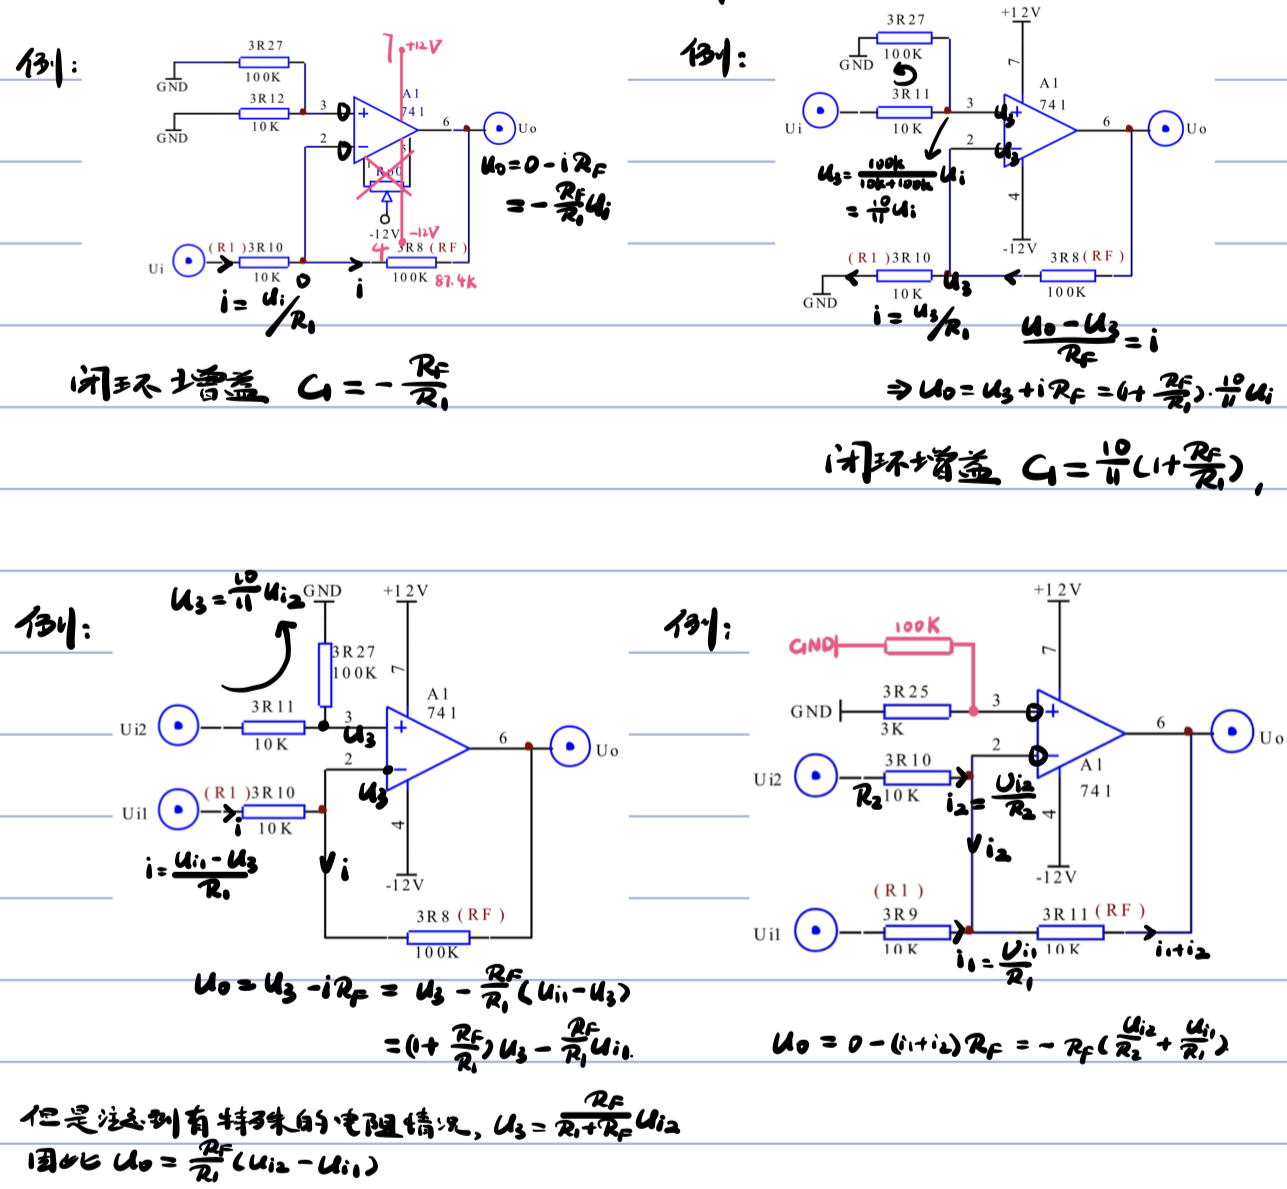
\includegraphics[width=\textwidth]{ET1_11GraP2.png}
		\caption{原理概述}
		\label{fig:figP2}
	\end{figure}
	
	计算所得理论值详见\textbf{实验结果展示}部分。
	
	% ---
	
	
	
	% 实验前思考题
	%\subsection{实验预习题}
	
	
	
	% ---
	
	
	
	% 实验记录	
	\clearpage
	
	% 顶栏
	\begin{table}
		\renewcommand\arraystretch{1.7}
		\centering
		\begin{tabularx}{\textwidth}{|X|X|X|X|}
			\hline
			专业: & 物理学 & 年级: & 2022级 \\
			\hline
			姓名: & 戴鹏辉、杨舒云 & 学号: & 22344016、22344020\\
			\hline
			室温: & 26\degree C & 实验地点: & A522 \\
			\hline
			学生签名:& 见\textbf{附件}部分 & 评分: &\\
			\hline
			实验时间:& 2024/6/19 & 教师签名:&\\
			\hline
		\end{tabularx}
	\end{table}
	% ---
	
	% 小标题
	\section{ET1-11 模拟运算放大电路  \quad\heiti 实验记录}
	% ---
	
	% 实验过程记录
	\subsection{实验内容、步骤与结果}
	
	%
	\subsubsection{操作步骤记录}
	\begin{enumerate}
		\item 反相比例放大器
		
		如\cref{fig:figR1}所示连接电路,按给定直流输入信号,测量对应的输出电压,记录结果。在该比例放大器的输入端加入1KHz, 有效值为0.5V的交流信号,用示波器观察输出波形,并与输入波形相比较。
		
		\begin{figure}[htbp]
			\centering
			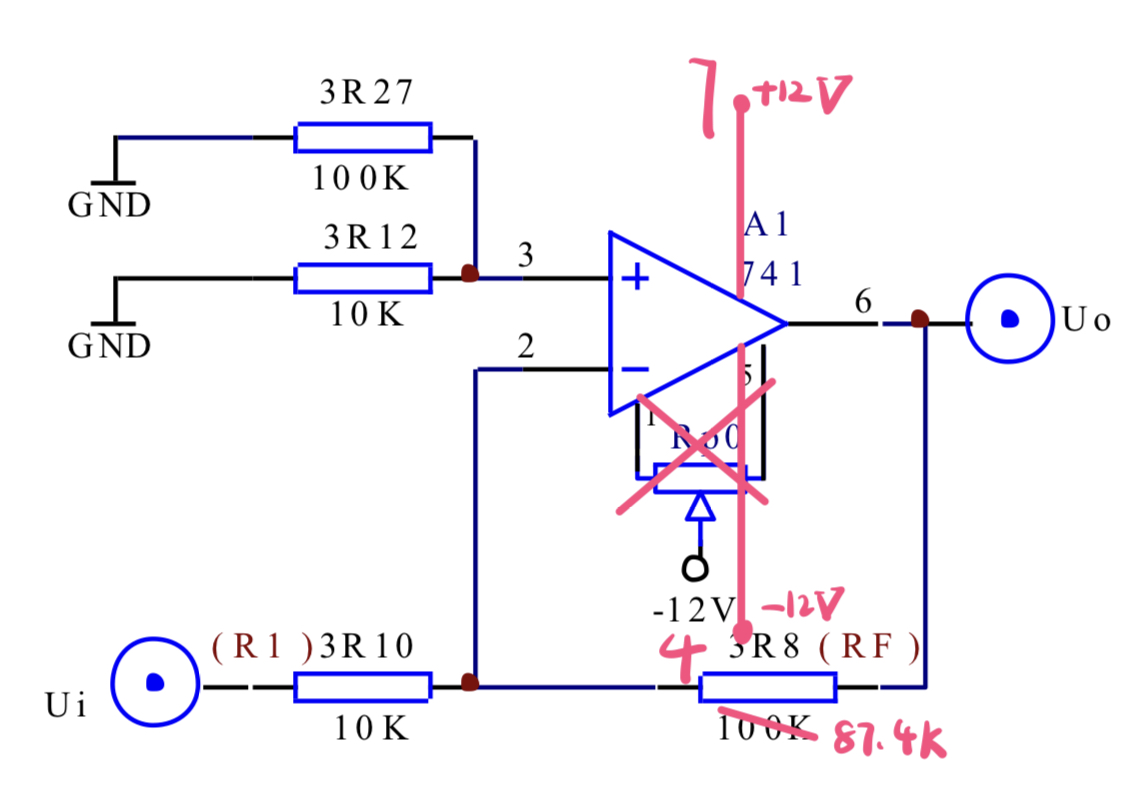
\includegraphics[width=0.5\textwidth]{ET1_11GraR1.png}
			\caption{反相比例放大器}
			\label{fig:figR1}
		\end{figure}
		
		\item 同相比例放大器
		
		如\cref{fig:figR2}所示连接电路。按给定直流输入信号,测量对应的输出电压,记录结果。在该比例放大器的输入端加入1KHz, 有效值为0.5V的交流信号,用示波器观察输出波形,并与输入波形相比较。
		
		\begin{figure}[htbp]
			\centering
			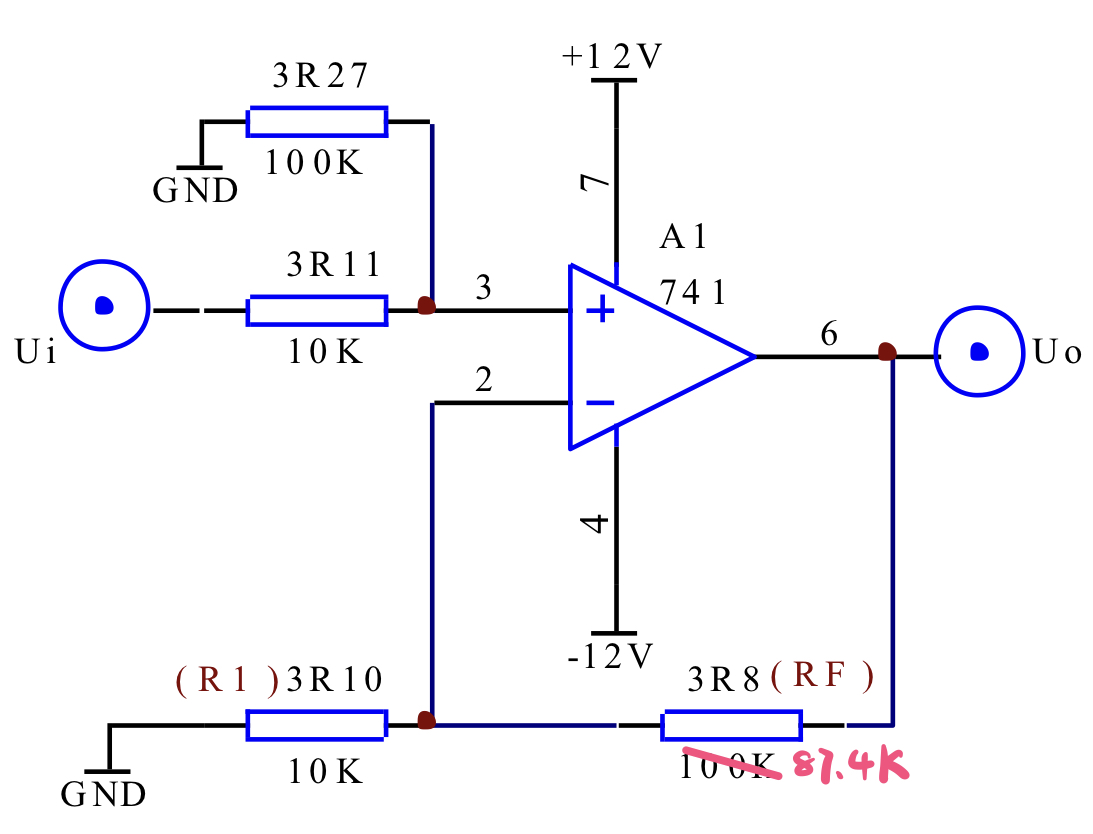
\includegraphics[width=0.5\textwidth]{ET1_11GraR2.png}
			\caption{同相比例放大器}
			\label{fig:figR2}
		\end{figure}
		
		\item 减法器(差分比例运算)
		
		如\cref{fig:figR3}所示连接电路。按给定直流输入信号,测量对应的输出电压,记录结果。
		
		\begin{figure}[htbp]
			\centering
			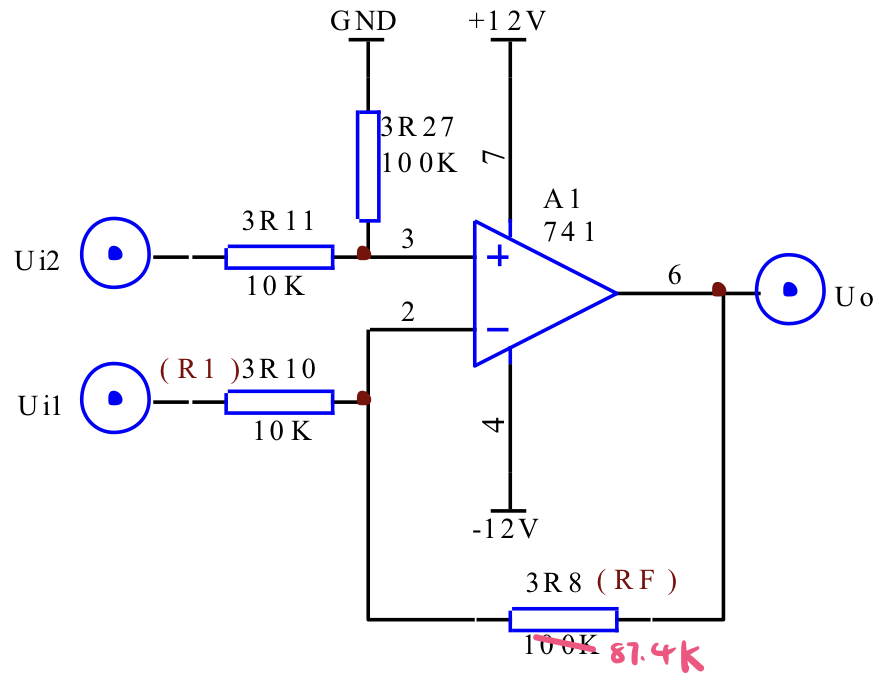
\includegraphics[width=0.5\textwidth]{ET1_11GraR3.png}
			\caption{减法器(差分比例运算)}
			\label{fig:figR3}
		\end{figure}
		
		\item 反相加法器
		
		如\cref{fig:figR4}所示连接电路。同时将Ui1与Ui2对地短路,接通电源后,调节调零电位器Rp0(10K),使输出Uo=0。然后将短路线去掉,按给定直流输入信号,测量对应的输出电压,记录结果。
		
		\begin{figure}[htbp]
			\centering
			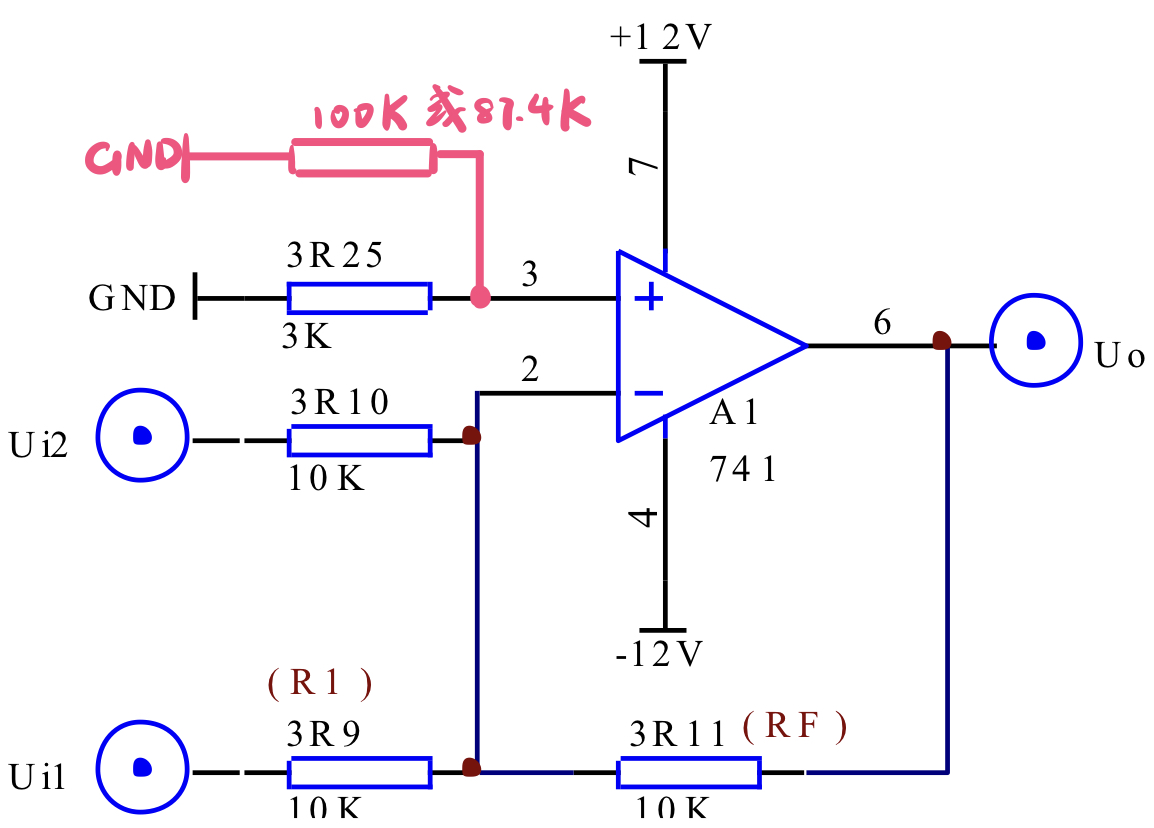
\includegraphics[width=0.5\textwidth]{ET1_11GraR4.png}
			\caption{反相加法器}
			\label{fig:figR4}
		\end{figure}
		
		\item 加减法器
		
		如\cref{fig:figR5}所示连接电路。将3R10与第一级运放的联接断开,按前述方法对两级分别进行调零。然后将短路线去掉,接好电路,按给定直流输入信号(Ui1和Ui2由同一信号源提供),测量对应的输出电压,记录结果。
		
		\begin{figure}[htbp]
			\centering
			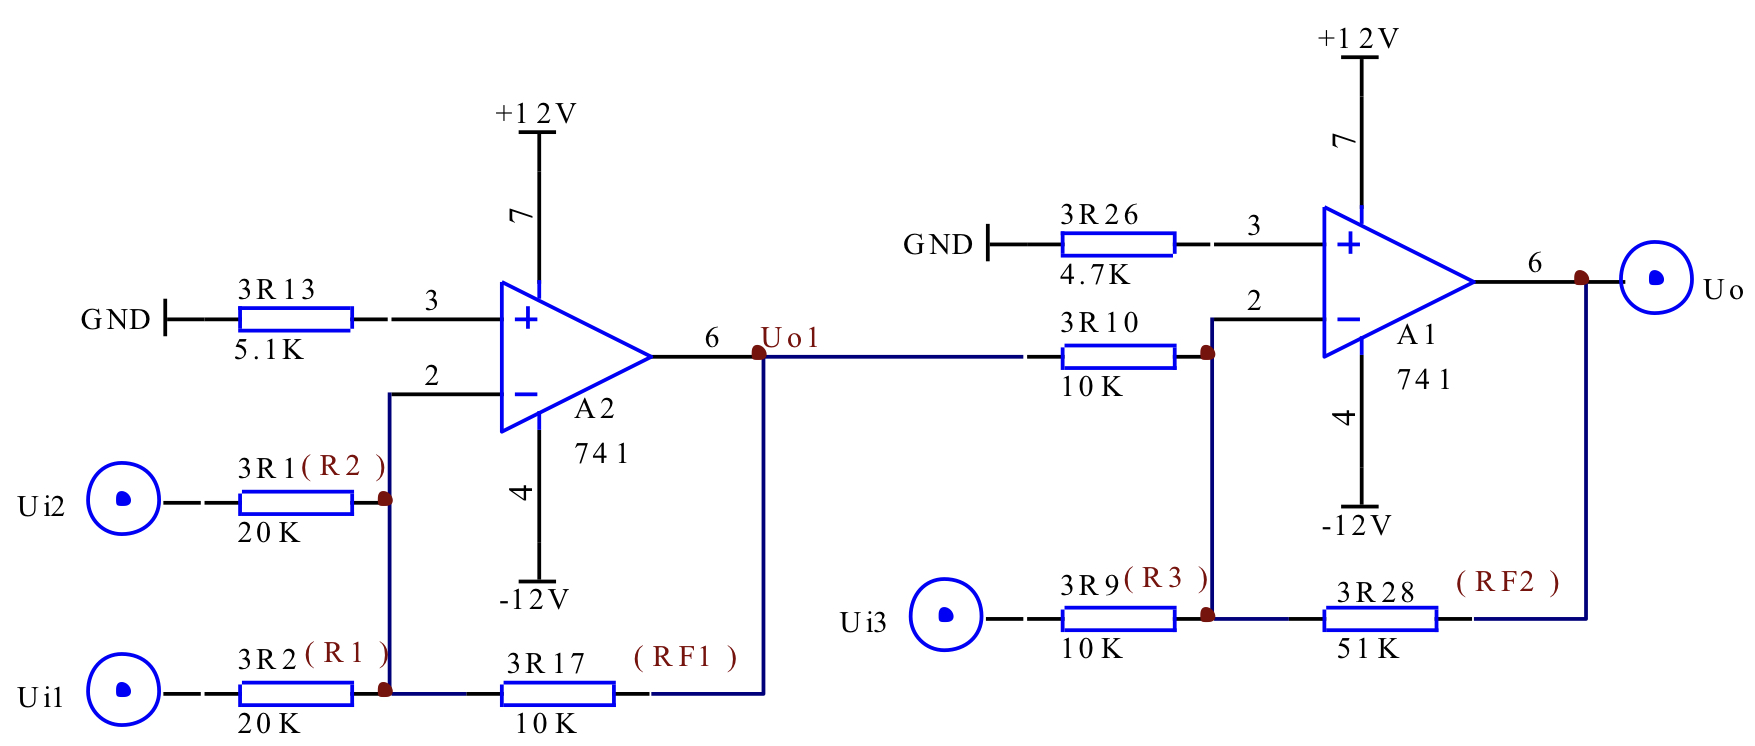
\includegraphics[width=0.5\textwidth]{ET1_11GraR5.png}
			\caption{反相加法器}
			\label{fig:figR5}
		\end{figure}
		
	\end{enumerate}	
	
	%
	\subsubsection{实验结果展示}
	\begin{enumerate}
		\item 反相比例放大器
		
		实验结果如\cref{tab:tab1}所示。波形图如\cref{fig:fig1}所示。
		
		\begin{table}[htbp]
			\centering
			\caption{实验数据:反相比例放大器}
			\label{tab:tab1}
			\begin{tabular}{|c|c|c|c|c|c|c|}
				\hline
				输入量 \( u_i \)/V & 0.3 & 0.5 & 0.7 & 1.0 & 1.1 & 1.2 \\
				\hline
				输出量理论值 \( u_o^{(T)} \)/V & -2.622 & -4.37 & -6.118 & -8.74 & -9.614 & -10.488 \\
				输出量实验值 \( u_o^{(E)} \)/V & -2.603 & -4.361 & -6.123 & -8.746 & -9.620 & -10.233 \\
				实测闭环增益 \( G \) & -8.68 & -8.72 & -8.75 & -8.75 & -8.75 & -8.53 \\
				相对误差 \( \eta \) & -0.72\% & -0.21\% & 0.08\% & 0.07\% & 0.06\% & -2.43\% \\
				\hline
			\end{tabular}
		\end{table}
		
		\begin{figure}[htbp]
			\centering
			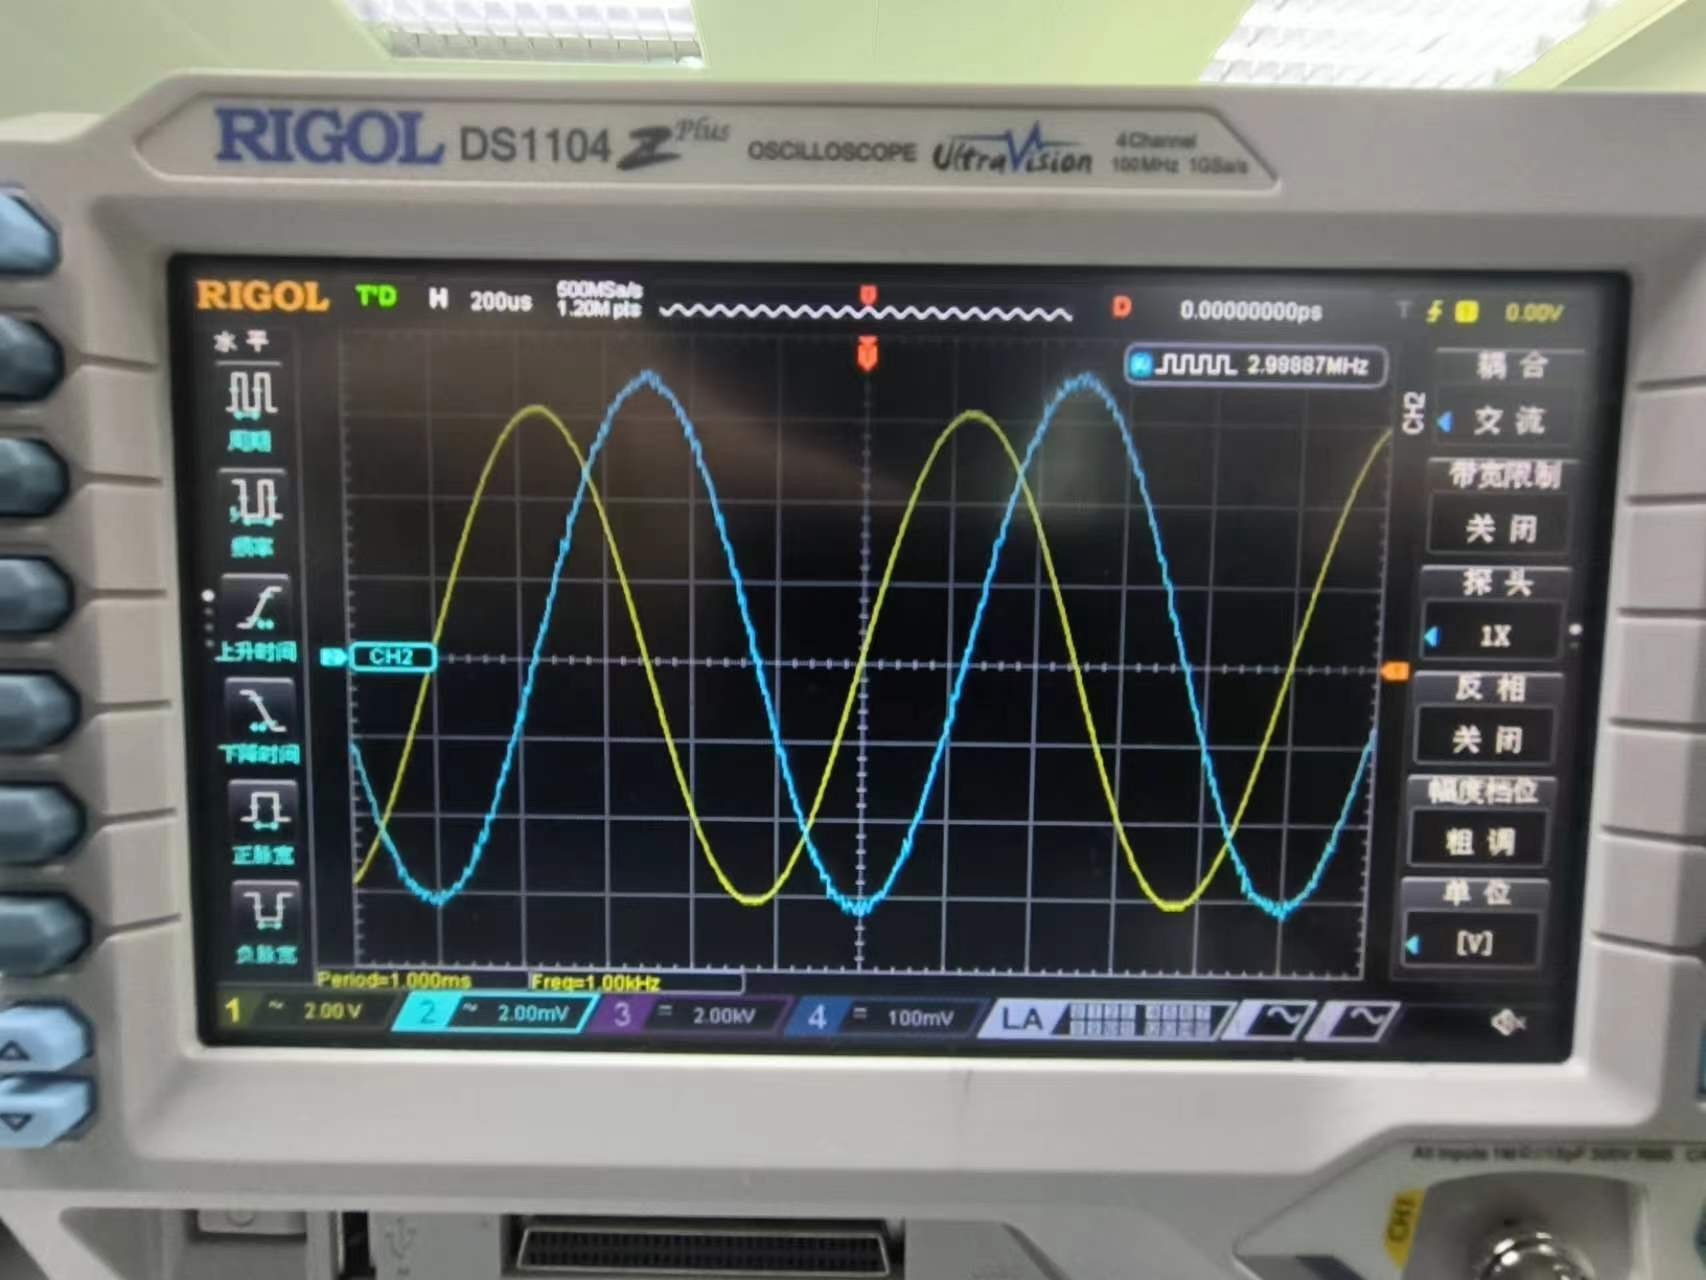
\includegraphics[width=0.5\textwidth]{反向比例放大器.jpg}
			\caption{波形图:反相比例放大器}
			\label{fig:fig1}
		\end{figure}		
		
		\item 同相比例放大器
		
		实验结果如\cref{tab:tab2}所示。波形图如\cref{fig:fig2}所示。
		
		\begin{table}[htbp]
			\centering
			\caption{实验数据:同相比例放大器}
			\label{tab:tab2}
			\begin{tabular}{|c|c|c|c|c|c|c|}
				\hline
				输入量 \( u_i \)/V & 0.3 & 0.5 & 0.7 & 1.0 & 1.1 & 1.2 \\
				\hline
				输出量理论值 \( u_o^{(T)} \)/V & 2.655 & 4.425 & 6.195 & 8.850 & 9.735 & 10.620 \\
				输出量实验值 \( u_o^{(E)} \)/V & 2.681 & 4.460 & 6.244 & 8.899 & 9.782 & 10.669 \\
				实测闭环增益 \( G \) & 8.94 & 8.92 & 8.92 & 8.90 & 8.89 & 8.89 \\
				相对误差 \( \eta \) & 0.98\% & 0.79\% & 0.79\% & 0.55\% & 0.48\% & 0.46\% \\
				\hline
			\end{tabular}
		\end{table}	
		
		\begin{figure}[htbp]
			\centering
			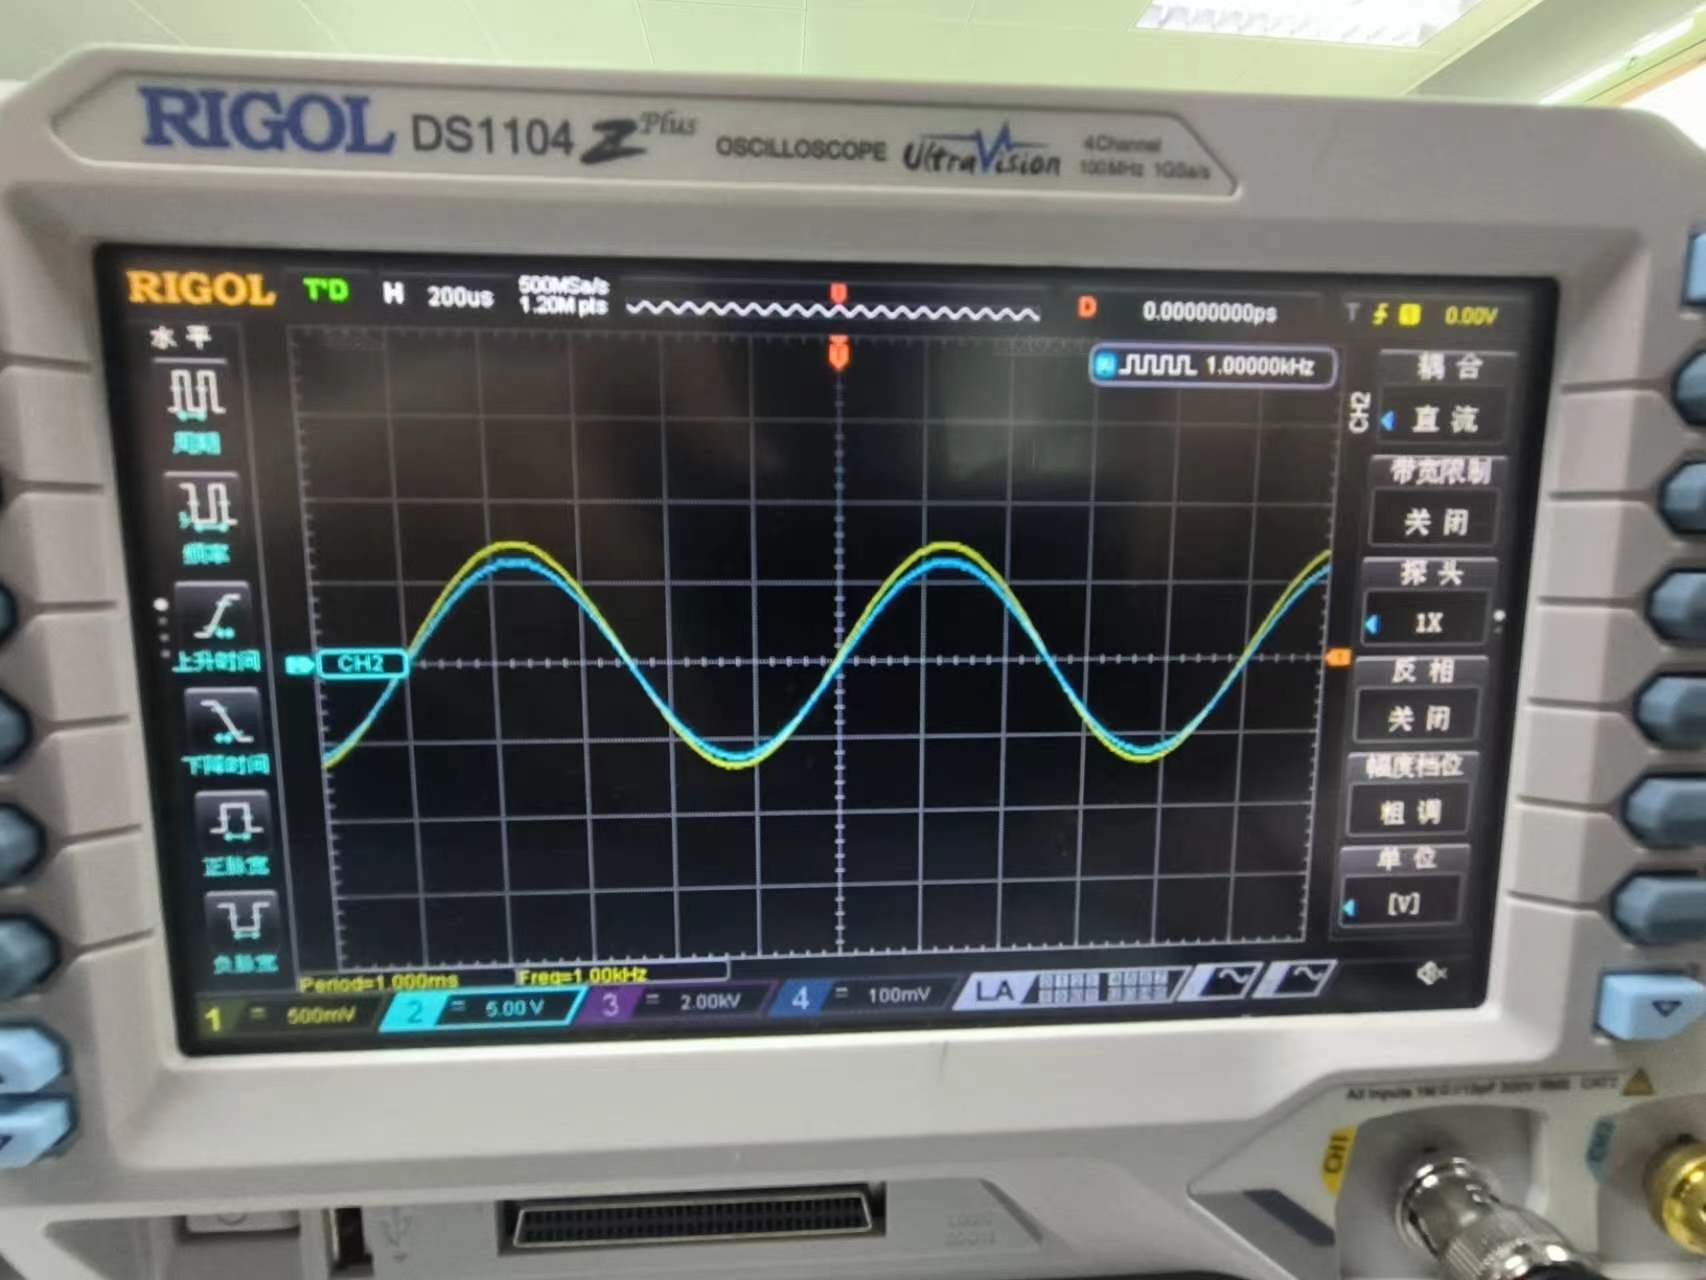
\includegraphics[width=0.5\textwidth]{同相比例放大器.jpg}
			\caption{波形图:同相比例放大器}
			\label{fig:fig2}
		\end{figure}	
		
		\item 减法器(差分比例运算)
		
		实验结果如\cref{tab:tab3}所示。
		
		\begin{table}[htbp]
			\centering
			\caption{实验数据:减法器(差分比例运算)}
			\label{tab:tab3}
			\begin{tabular}{|c|c|c|c|}
				\hline
				输入量 \( u_{i1} \)/V & 0.2 & 0.2 & -0.2 \\
				输入量 \( u_{i2} \)/V & -0.3 & 0.3 & -0.3 \\
				输出量理论值 \( u_o^{(T)} \)/V & -4.370 & 0.874 & -0.874 \\
				输出量实验值 \( u_o^{(E)} \)/V & -4.381 & 0.926 & -0.878 \\
				相对误差 \( \eta \) & 0.25\% & 5.95\% & 0.46\% \\
				\hline
			\end{tabular}
		\end{table}
		
		\item 反相加法器
		
		实验结果如\cref{tab:tab4}所示。
		
		\begin{table}[htbp]
			\centering
			\caption{实验数据:反相加法器}
			\label{tab:tab4}
			\begin{tabular}{|c|c|c|c|}
				\hline
				输入量 \( u_{i1} \)/V & 1.0 & 1.5 & -0.2 \\
				\hline
				输入量 \( u_{i2} \)/V & 0.4 & -0.4 & 1.2 \\
				\hline
				输出量理论值 \( u_o^{(T)} \)/V & -1.400 & -1.100 & -1.000 \\
				\hline
				输出量实验值 \( u_o^{(E)} \)/V & -1.382 & -1.089 & -0.981 \\
				\hline
				相对误差 \( \eta \) & -1.29\% & -1.00\% & -1.90\% \\
				\hline
			\end{tabular}
		\end{table}
		
		\item 加减法器
		
		实验结果如\cref{tab:tab5}所示。除此以外,计算得到相对误差$\eta=-1.80\%$。
		
		\begin{table}[htbp]
			\centering
			\caption{实验数据:加减法器}
			\label{tab:tab5}
			\begin{tabular}{|c|c|c|}
				\hline
				\( u_{i1} \)/V & \( u_{i2} \)/V & \( u_{i3} \)/V \\
				\hline
				0.398 & 0.775 & 0.401 \\
				\hline
				\( R_1 \)/k\(\Omega\) & \( R_2 \)/k\(\Omega\) & \( R_3 \)/k\(\Omega\) \\
				\hline
				20 & 20 & 10 \\
				\hline
				\( R_F \)/k\(\Omega\) & \( u_o^{(T)} \)/V & \( u_o^{(E)} \)/V \\
				\hline
				51 & 0.946 & 0.929 \\
				\hline
			\end{tabular}
		\end{table}
		
	\end{enumerate}	
	
	% ---
	
	% 原始数据
	\clearpage
	\subsection{原始数据记录}
	实验记录本上的原始数据见\cref{fig:figO1}与\cref{fig:figO2}(签字)。
	
	\begin{figure}[htbp]
		\centering
		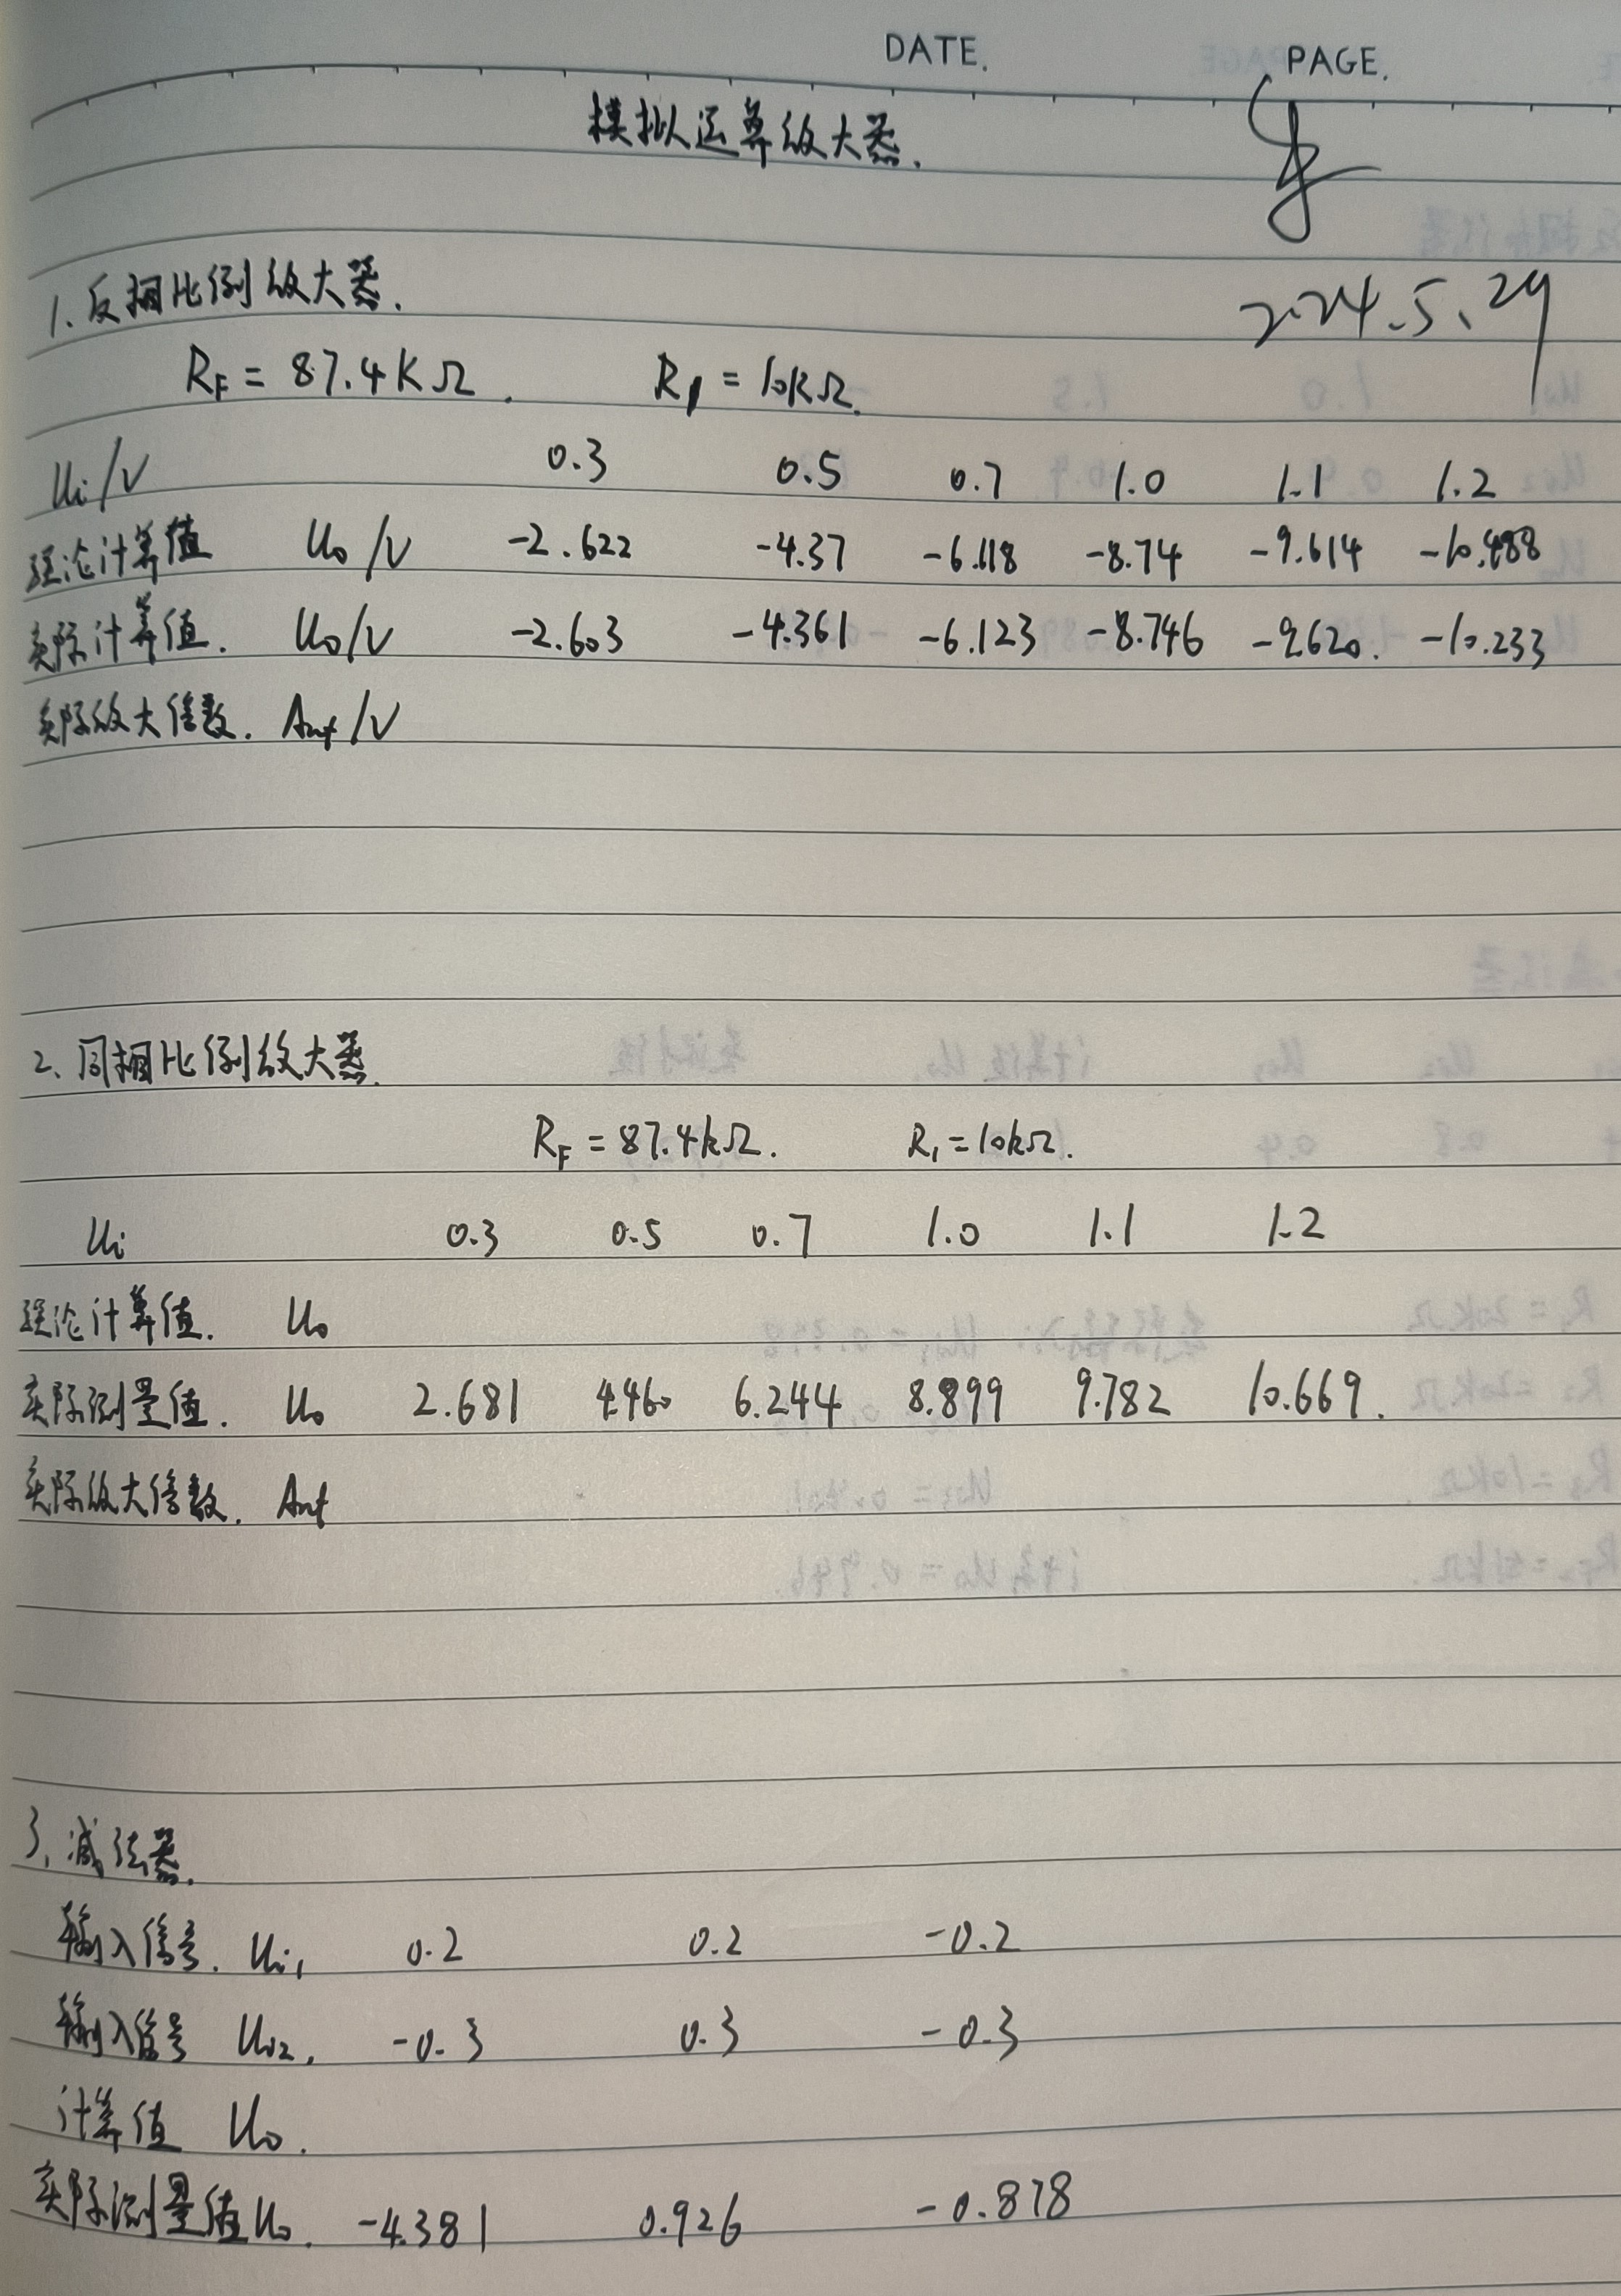
\includegraphics[width=0.38\textwidth]{ET1_11GraO1.jpg}
		\caption{原始数据记录1}
		\label{fig:figO1}
	\end{figure}
		
	\begin{figure}[htbp]
		\centering
		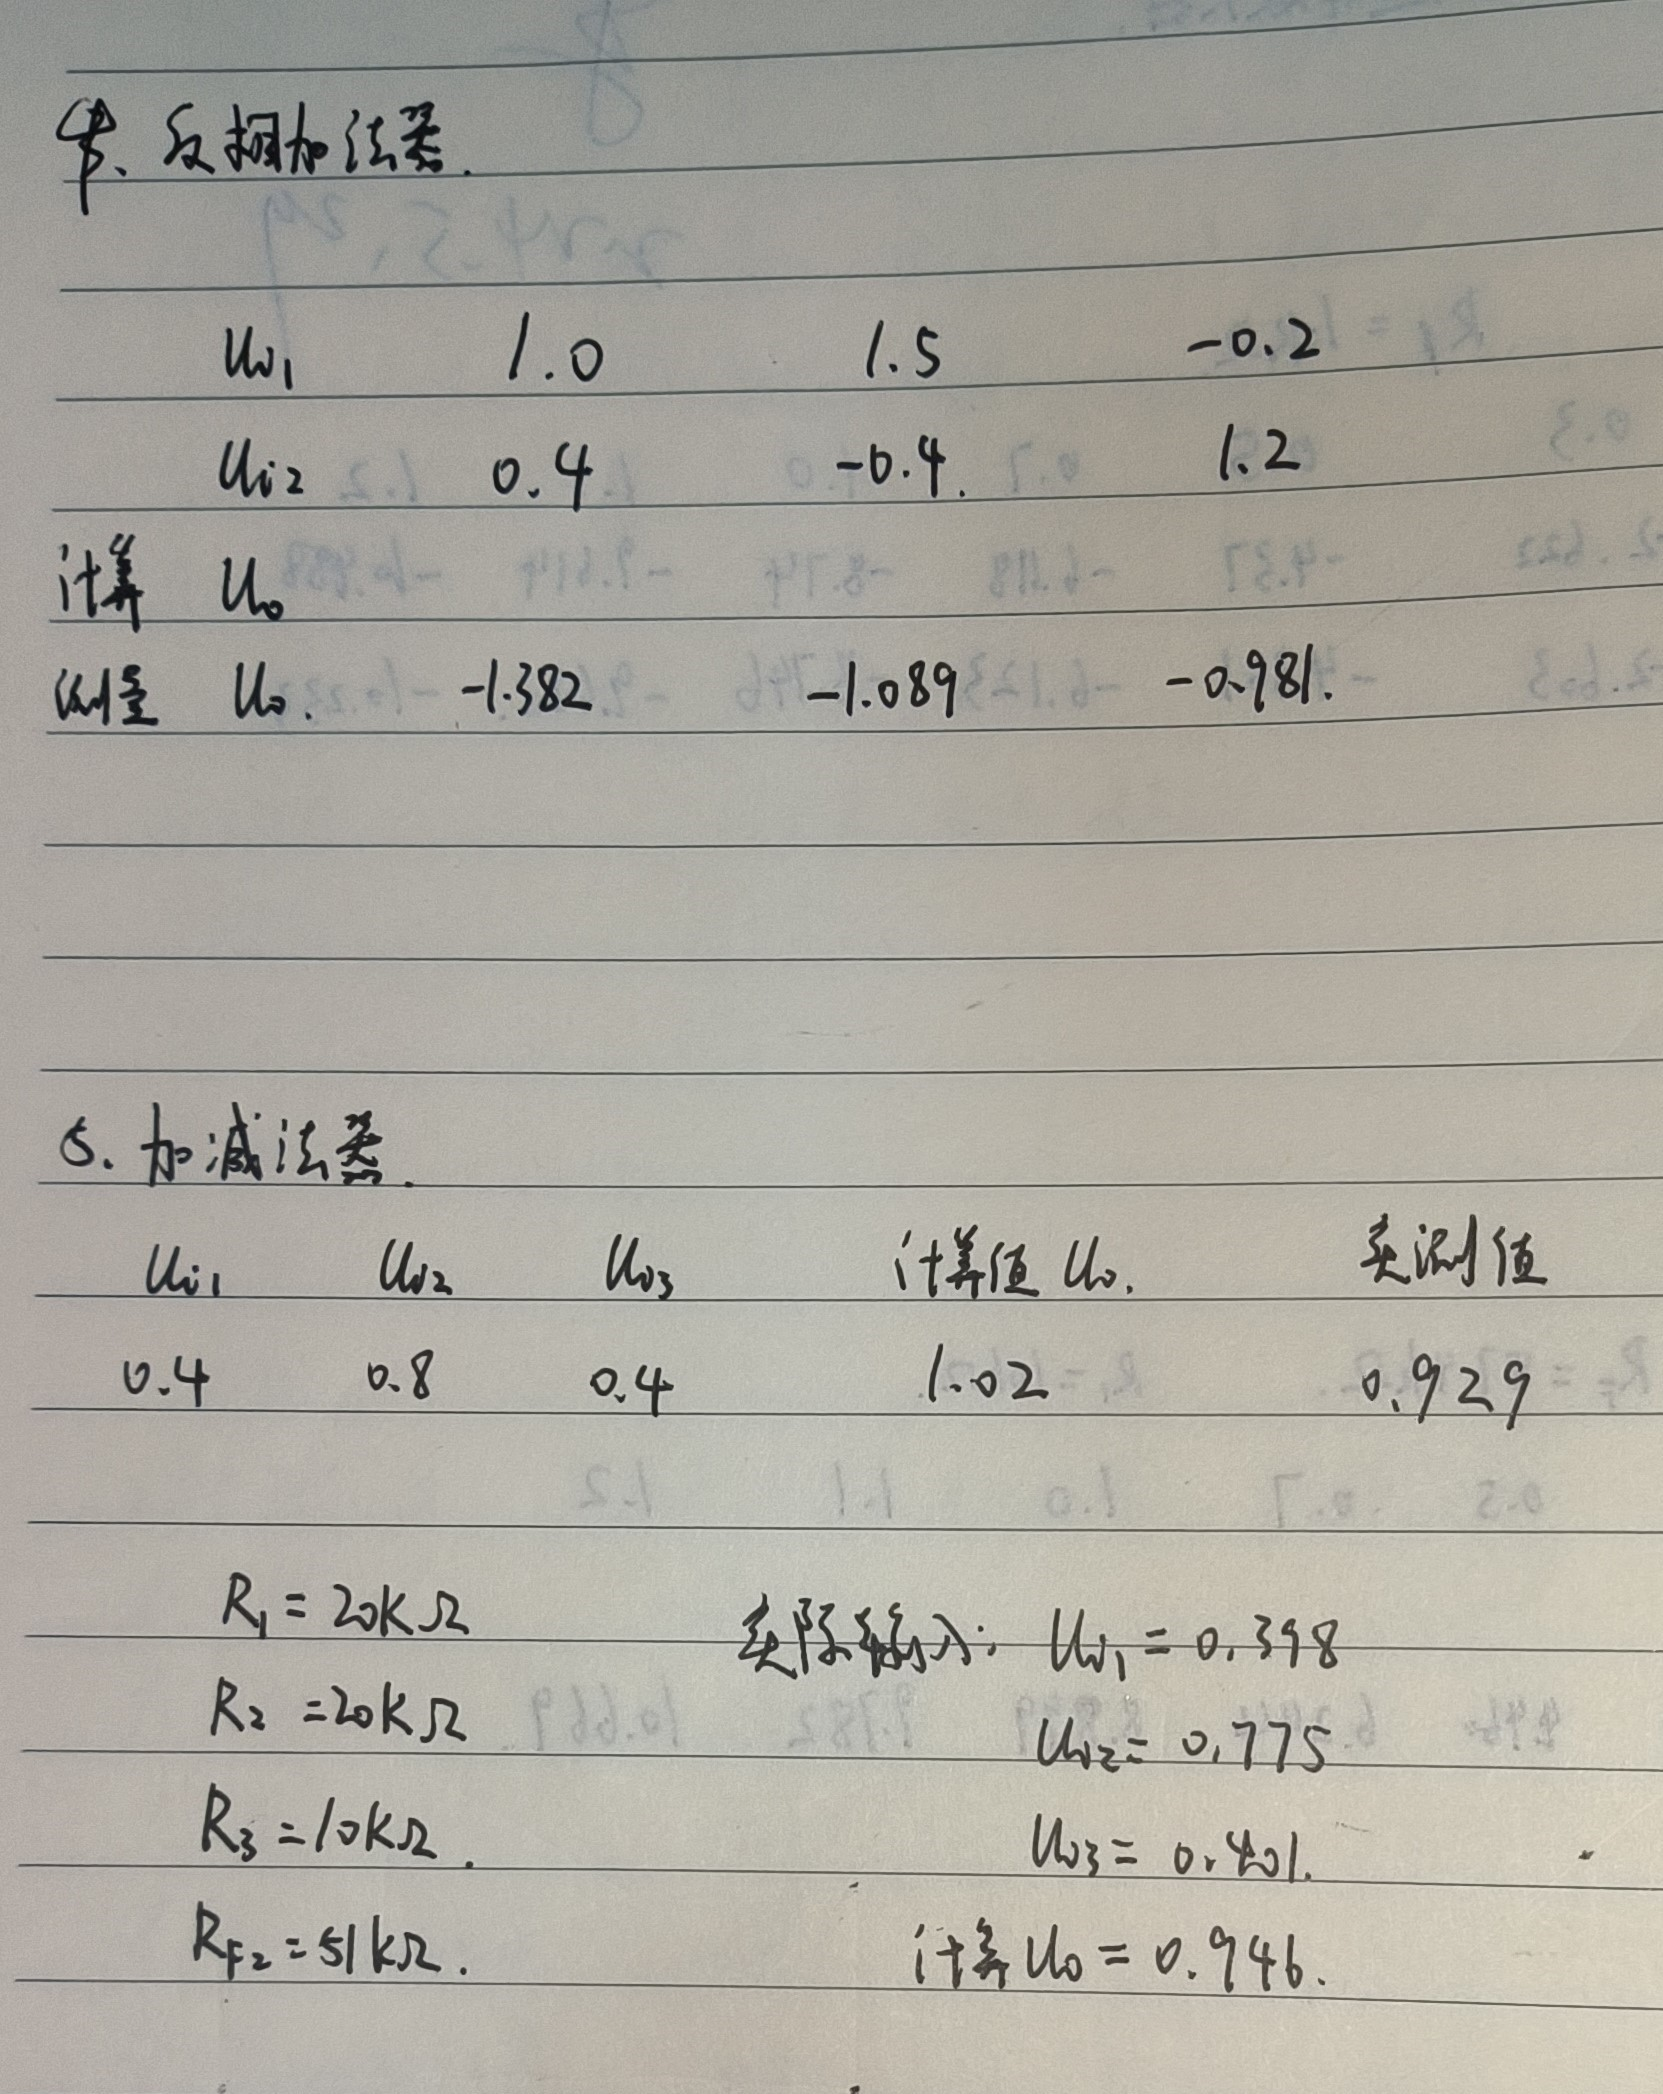
\includegraphics[width=0.28\textwidth]{ET1_11GraO2.jpg}
		\caption{原始数据记录2}
		\label{fig:figO2}
	\end{figure}
	
	%实验台桌面整理见%\textbf{附件}部分(\cref{})。
	
	%其它原始数据见%\cref{}。
	% ---
	
	% 问题记录
	%\subsection{实验过程遇到问题及解决办法}
	
	% ---
	
	
	
	% 分析与讨论	
	\clearpage
	
	% 顶栏
	\begin{table}
		\renewcommand\arraystretch{1.7}
		\begin{tabularx}{\textwidth}{|X|X|X|X|}
			\hline
			专业:& 物理学 &年级:& 2022级\\
			\hline
			姓名: & 戴鹏辉、杨舒云 & 学号:& 22344016、22344020\\
			\hline
			日期:& 2024/6/19 & 评分: &\\
			\hline
		\end{tabularx}
	\end{table}
	% ---
	
	% 小标题
	\section{ET1-11 模拟运算放大电路 \quad\heiti 分析与讨论}
	% ---
	
	% 数据处理
	\subsection{实验数据分析}
	
	数据分析这个一部分主要讨论关于实验值与理论值得误差来源。我们可以作如下考虑。
	
	\begin{enumerate}
		\item 有限开环增益的影响
		
		由于我们计算理论值时假定了开环增益时无穷大,然而实际运放的开环增益只是非常大,并不是无限的,这可能会带来一些误差。具体计算细节如\cref{fig:figA1}与\cref{fig:figA2}所示,参考了文献[3]。
		
		\begin{figure}[htbp]
			\centering
			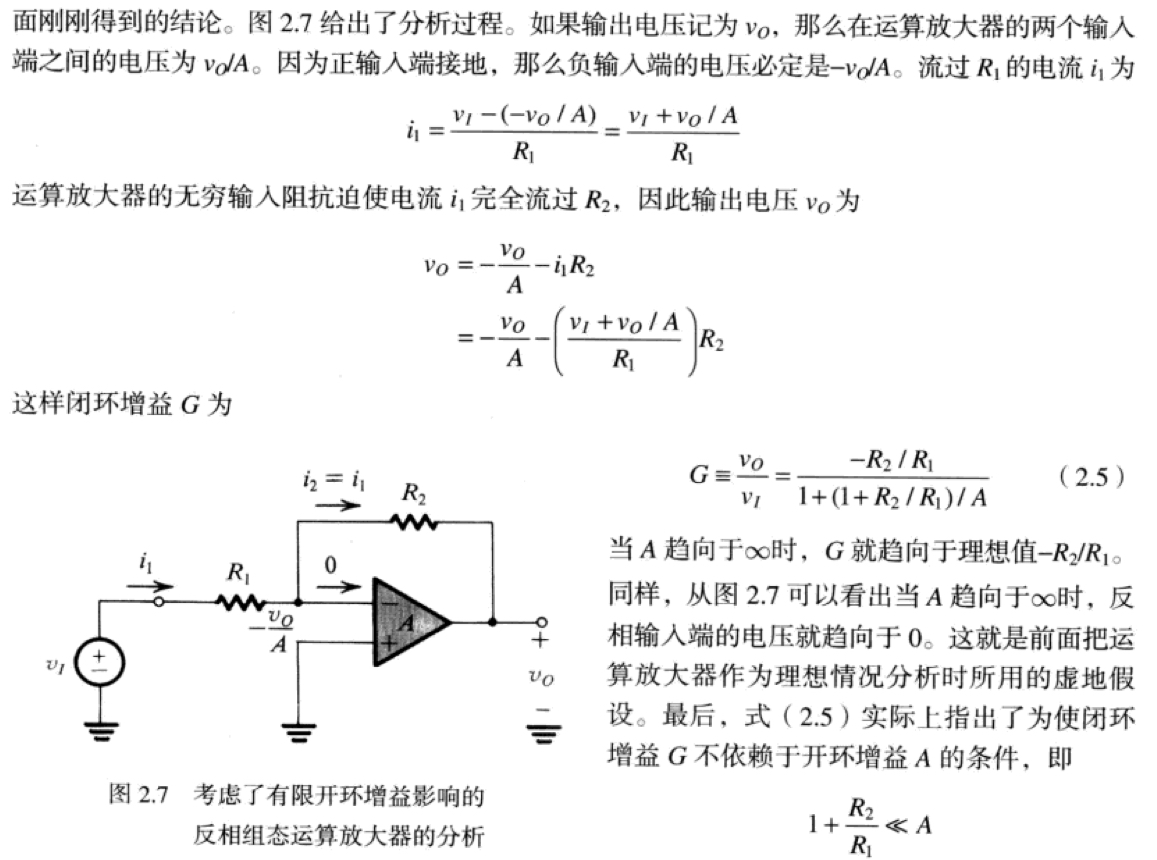
\includegraphics[width=\textwidth]{ET1_11GraA1.png}
			\caption{有限开环增益的影响:反相组态}
			\label{fig:figA1}
		\end{figure}
		
		\begin{figure}[htbp]
			\centering
			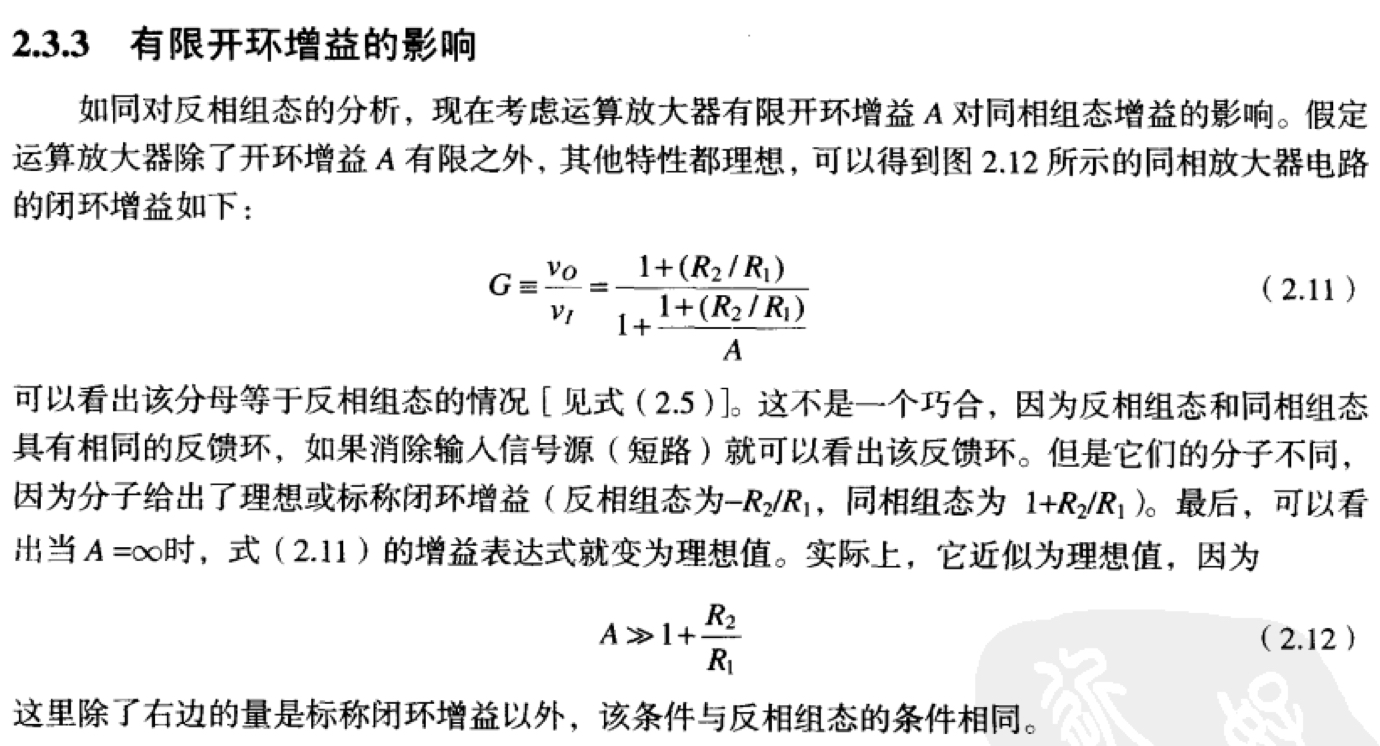
\includegraphics[width=\textwidth]{ET1_11GraA2.png}
			\caption{有限开环增益的影响:同相组态}
			\label{fig:figA2}
		\end{figure}
		
		\item 电源实际输出电压
		
		事实上,我们将直流电源设定为实验要求值之后,事实上的输出电压并不真的是该值,甚至有着较大差异,这一点在加减法器实验中表现得尤为明显,具体可以参见测量结果。
		
		\item 其它因素
		
		元件公差:电路中使用的电阻和其他元件都有自己的公差值,这可能导致电路实际参数与设计参数有所不同,从而影响输出结果。
		
		运算放大器的非理想特性:例如,741运算放大器的输入偏置电流、输入偏置电压、增益带宽积等非理想特性都可能影响电路的性能。这些特性在高频或高负载条件下可能更加明显。
		
		布线和接地问题:电路的布线长度、布线方式以及接地的质量都会影响电路的性能。例如,长的布线可能引入额外的电感和电容效应,而接地不良可能引起信号干扰和噪声问题。
		
		温度和环境因素:电阻和运算放大器的参数可能会随环境温度变化而变化,这种变化可能没有在理论计算中考虑。
		
		除此以外,思考题中也提供了一部分误差来源的分析,详见思考题。
	\end{enumerate}
	
	% 实验后思考题
	\subsection{实验思考题}
	
	%思考题1
	\begin{question}
		运算放大器作比例放大时,R1与RF的阻值误差为$\pm 10 \%$,试问如何分析和计算电压增益的误差?
	\end{question}
	1. 为了分析增益的变化范围,我们需要计算出在阻值误差范围内可能出现的最大和最小增益值。这可以通过分别代入\( R_F \)和\( R_1 \)的最大和最小可能值来计算:
	
	\( R_F \)的最大值为\( 1.1R_F \),最小值为\( 0.9R_F \);\( R_1 \)的最大值为\( 1.1R_1 \),最小值为\( 0.9R_1 \)。
	
	因此,最大和最小增益可以分别计算为:
	\[ A_{v,\text{max}} = -\frac{0.9R_F}{1.1R_1} \]
	\[ A_{v,\text{min}} = -\frac{1.1R_F}{0.9R_1} \]
	
	通过上述计算得到的最大和最小增益值,可以得到增益的误差范围。
	
	增益的相对误差可以通过比较最大增益和最小增益与理论增益的差异来估计:
	\[ \text{相对误差} = \frac{A_{v,\text{max}} - A_v}{A_v} \times 100\% \]
	\[ \text{相对误差} = \frac{A_{v,\text{min}} - A_v}{A_v} \times 100\% \]
	
	% 思考题2
	\begin{question}
		运算放大器作精密放大时,同相输入端对地的直流电阻要与反相输入端对地的直流电阻相等,如果不相等,会引起什么现象?
	\end{question}
	在运算放大器(Op-Amp)的应用中,尤其是在精密放大器设计时,确保同相输入端(非反相端,+端)和反相输入端(-端)对地的直流电阻相等是非常重要的。这种匹配主要是为了减少和消除两种潜在问题:
	
	\begin{enumerate}
		\item 输入偏置电流产生的电压偏移:运算放大器的两个输入端都有小的输入偏置电流。当同相端和反相端的电阻匹配时,由于这两个电流通过相等的电阻流过,它们在两端产生的电压降是相同的,这有助于抵消电流产生的电压偏移。如果这两个电阻不匹配,每个端子的电压降将不同,导致输入端出现一个额外的电压偏差,这个偏差将被放大器放大,从而影响输出精度。
		
		\item 共模噪声抑制的降低:在理想情况下,运算放大器能够完美地抑制两个输入端上相同的共模信号(即同时出现在同相端和反相端的信号)。但如果两端对地的直流电阻不同,共模噪声抑制比(Common-Mode Rejection Ratio, CMRR)会降低。这是因为不平衡的电阻会导致运算放大器在处理共模信号时的不对称响应,增强了共模噪声在输出中的影响。
	\end{enumerate}
	
	因此,如果同相端和反相端对地的直流电阻不相等,最主要的影响是增加了输出信号中的偏差和噪声,这对于需要高精度的应用(如精密测量、音频处理等)是不可接受的。这就需要设计时仔细选择和匹配这些电阻,以确保高性能和准确性。
	
	% ---
	
	
	% 结语部分
	\clearpage
	
	% 小标题
	\section{ET1-11 模拟运算放大电路 \quad\heiti 结语}
	% ---
	
	% 总结、杂谈与致谢
	%\subsection{实验心得和体会、意见建议等}
	
	% ---
	
	% 参考文献
	\subsection{参考文献}
	[1] 维基百科 https://zh.wikipedia.org
	
	[2] 电子技术实验讲义
	
	[3] 微电子电路
	
	% ---
	
	% 附件
	\subsection{附件及实验相关的软硬件资料等}
	%试验台桌面整理如%\cref{}所示。
	
	实验报告个人签名如\cref{fig:name}。
	
	\begin{figure}[htbp]
		\centering
		\subfloat[]{
			
\includegraphics[width=0.45\textwidth]{name.png}
		}
		\subfloat[]{
			
\includegraphics[width=0.45\textwidth]{name-TaLEs.jpg}
		}
		\caption{个人签名}
		\label{fig:name}			
	\end{figure}
	
	% ---
	
	相关代码已上传至Github。
	
	
	
\end{document}